\documentclass[]{article}

\usepackage{algorithm}
\usepackage{algorithmic}
\usepackage{amsmath}
\usepackage{amssymb}
\usepackage{amsthm}
\usepackage[ngerman,english]{babel}
\usepackage{centernot} 
\usepackage{color}
\usepackage{dsfont}
\usepackage{graphicx}
\usepackage[utf8]{inputenc}
\usepackage{import}
\usepackage{standalone}
\usepackage{qtree}

\usepackage{hyperref}

\title{SOP Challenge - Presentation}
\author{TBD}

\newcommand{\N}{\ensuremath{\mathds{N}}}
\newcommand{\R}{\ensuremath{\mathds{R}}}
\newcommand{\red}[1]{\textcolor{red}{#1}}

\setlength{\itemsep}{-2pt}


\begin{document}
    \maketitle
    \tableofcontents


    %\import{files/}{example_1.tex}

    \section{SOP Problem}

    The Sequential Ordering Problem (SOP) is an asymmetrical TSP with precedence constraints. 

    Each instance of this problem consists of a directed graph $G=(V, A)$, arc weights $w: A \rightarrow \mathbb{R}$, a set of precedence constraints $C \subset V \times V$ as well as a start vertex $s$ and destination vertex $t$.

    The problem consists in finding a permutation of vertices starting at s, ending at t, which satisfy all precedence constraints and minimize the weighted sum of arcs connecting the vertices in the given order. \cite{libralesso2019tree}

    \begin{figure}[hbt]
    	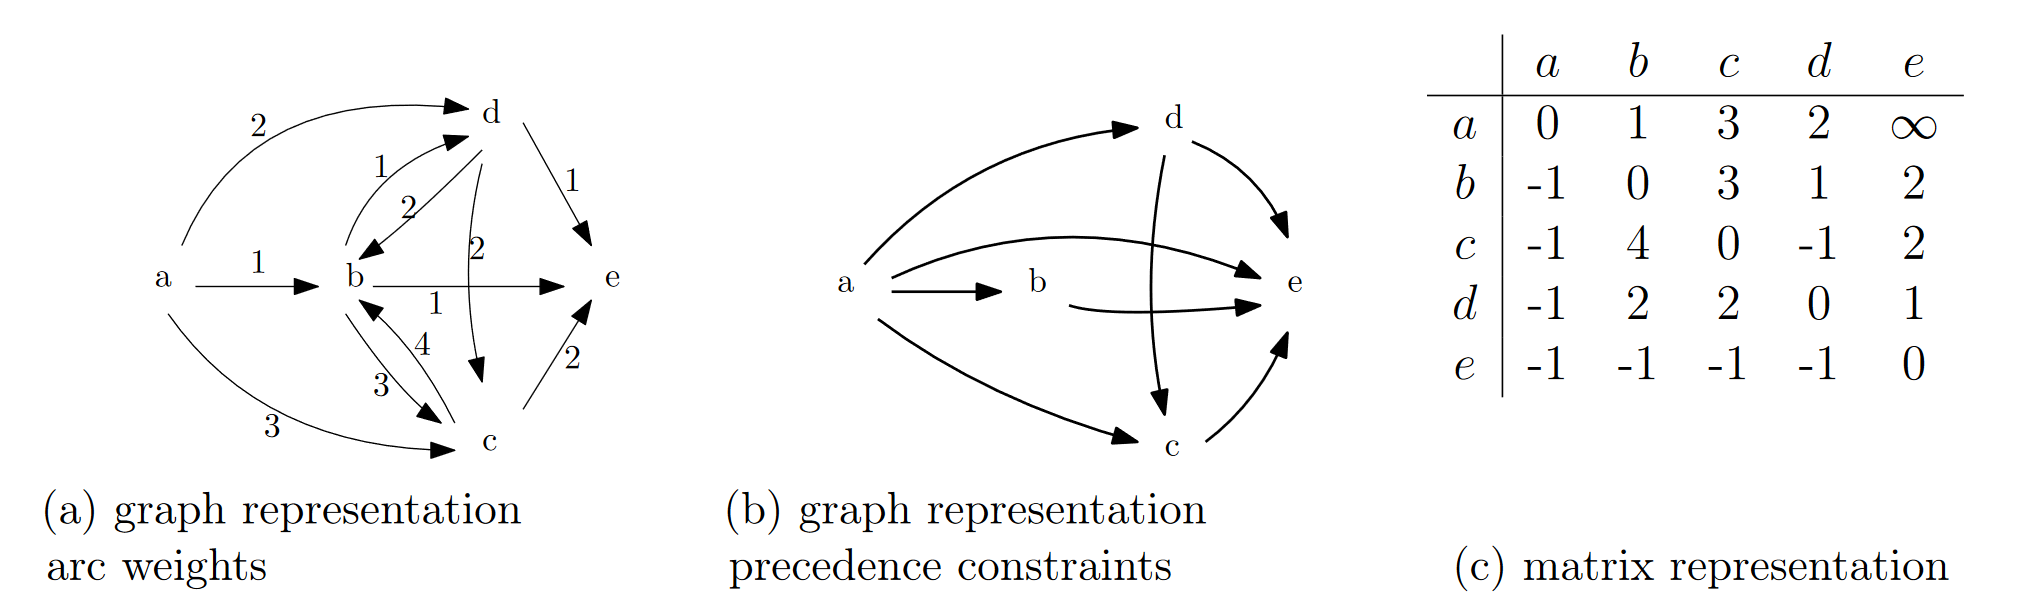
\includegraphics[width=\textwidth]{files/graphic_sop_prob.png}
    	\centering
    	\caption{Illustrative example \cite{libralesso2019tree}}
    \end{figure}



    \section{Solution approaches}

    \subsection{Implemented methods}

    We have implemented multiple methods for solving the SOP Challenge namely an Exact Method and Particle Swarm Optimization Method as well as a 
    Greedy Method and closely related variations of it. In the following we will discuss the latter methods since they have turned out to be the most 
    stable methods in terms finding feasible solutions and computation time in our experiments. We will now give a short description of each of the 
    methods. Tables with results for each of the methods can be found in \ref{results}.
    
    \subsubsection{Discrete Particle Swarm Optimization (DPSO)}
    
    PSO is a population based algorithm that is trying to iteratively improve all candidate solutions (particles) in the population. At every 
    iteration, each particle is influenced by its local position, it is also guided towards his personal best position and, most important, by the 
    best global position found by the entire swarm so far. Each particle updates its personal best position, while the global best position is 
    updated by all particles. There are some parameters that influence local, personal and global updates and they should be optimized. The 
    population size and number of iterations directly impact the running time of the algorithm. The power of this approach comes from the random 
    that is introduced in the update equations. This is the mechanism that makes one particle jump out of a local minima (or a plateau) and continue 
    exploring the space of solutions while still taking into account its personal best and global best. In order to have better understanding about 
    how this algorithm works, \href{https://upload.wikimedia.org/wikipedia/commons/e/ec/ParticleSwarmArrowsAnimation.gif}{click here.}.\\
    
	In the continuous case presented above, it is guaranteed that changes applied to each particle lead to a feasible solution. For 
	example, when our search space is $ \mathbb{R}^n $, the update equation generates a solution that is also in $ \mathbb{R}^n $. Well, this is not 
	true for the discrete case and this is the problem that leads to some modifications of PSO for continuous case.\\
	
	In order to apply DPSO for SOP Problem, new update rules need to be derived in order to generate a feasible solution at each iteration. We 
	implemented DPSO version presented in paper \cite{DPSO-paper} where the authors design operations for updates at each iteration. For SOP Problem, 
	each particle is represented by a permutation where first and last nodes are fixed. We need to make sure the operations applied to each 
	permutation (particle) lead to a valid permutation for our problem, which means that it should respect the precedence constraints. Before 
	evaluating the cost of a particle (permutation), we need to make sure the particle respects the precedence constraints. If it doesn't, then it is 
	passed to a procedure that changes it in order to respect the constraints. This is the point of DPSO that is time-consuming especially for big 
	instances, such as "R.n.r.p" instances. Once we make sure we generate feasible particle at teach iteration, we need to let DPSO procedure to find 
	permutations with smaller and smaller costs. \\
	
	Our implementation serializes the DPSO object in order to load it later and continue optimization. Normally, (D)PSO is usually implemented 
	without any parallelization support, but we decided to use multiprocessing for each iteration in order to speed-up the computation because the 
	prodecure of forcing the particle to respect precedence constraints is time consuming. \\
	
	In order to have a powerful (D)PSO algorithm, we would need a reasonably big swarm (a few tens, up to one hundred or two), but given the fact 
	that some problems are big, we could only use a small swarm size. For example, for big problems where $ n > 65 $, we could only use one swarm per 
	CPU core. On the computer that we run the experiments on, we used 7 cores and finally had 7 particles to explore a big space. We remind that for 
	big values of $ n $ the procedure of fixing the particle is very slow.
	
    \subsubsection{Greedy Method}

   	The first, simple heuristic we implemented was a greedy algorithm for the SOP Problem. The Greedy algorithm builds a solution starting from the initial node by choosing the the next best node in terms of cost and precedence constraints. As should be known the greedy algorithm makes local optimal decision which not always lead global optimal solutions. Furthermore the greedy algorithm was able to find feasible solutions for all instances quite fast and is easily implemented due to the local search criteria. \cite{Cormen2009} \\

   	In the case of the SOP Problem the greedy algorithm starts the generation of the Hamiltonian path at the initial node. At each iteration of the 
   	algorithm we compute the set of unvisited nodes which do not violate the precedence constraints given by the instance. We then append the node 
   	with the lowest cost (greedy selection) for this set to the current path. This procedure repeats until all nodes have been visited and the final 
   	node has been reached.

    \subsubsection{Beam Search Method}

    The idea of beam search, in contrast to the greedy algorithm, is to build $K$ different solutions in parallel, where $K$ is called the beam width. For the SOP Problem the algorithms initializes all solution paths from the initial node. It then finds all possible children of the node(s) and computes the cost of each of the new potential paths. To maintain the beam width it selects the $K$ best new paths and repeats these steps until all nodes have been visited and the end vertex has been reached. \cite{Beam:1} \cite{Beam:2} 

    \begin{figure}[hbt]
    	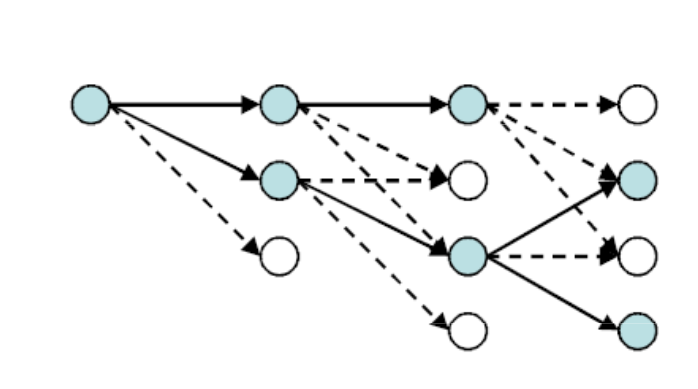
\includegraphics[]{files/beam_search.png}
    	\centering
    	\caption{Beam Search}
    \end{figure}

    \TODO{Add description}

    \subsection{Results}
    \label{results}

    The subsequent tables contain results for the used methods. The first table (\ref{table:results_cost}) displays the costs of the found solutions the second table (\ref{table:results_time}) the time needed to compute the solutions.
    
    BS10 refers to a beam search of width 10 and BSV to a beam search of width $|V|$.

    \begin{table}[htb]
		\rowcolors{2}{gray!25}{white}
		\begin{tabular}{lcccccc}
			Instance       & LB     &    UB      & DPSO   &   Greedy &   BS10   &   BSV   \\
			ESC07          & 2125   &    2125    & 2125   &   2700   &   2125   &   2125  \\
			ESC11          & 2075   &    2075    & 2195   &   3175   &   2480   &   2480  \\
			ESC12          & 1675   &    1675    & 1675   &   2034   &   2429   &   1997  \\
			ESC25          & 1681   &    1681    & 6518   &   3360   &   2010   &   1821  \\
			ESC47          & 1288   &    1288    & 11617  &   3843   &   2186   &   2664  \\
			ESC63          & 62     &    62      & 185    &   76     &   72     &   67    \\
			ESC78          & 18230  &    18230   & 27900  &   22600  &   20425  &   20340 \\
			kro124p.1      & 38762  &    39420   & -      &   52575  &   49074  &   49680 \\
			kro124p.2      & 39841  &    41336   & -      &   57723  &   54185  &   52568 \\
			kro124p.3      & 43904  &    49499   & -      &   77266  &   64330  &   60999 \\
			kro124p.4      & 73021  &    76103   & -      &   98427  &   94773  &   89152 \\
			ry48p.1        & 15805  &    15805   & 39933  &   22493  &   17739  &   18888 \\
			ry48p.2        & 16074  &    16666   & 40867  &   20911  &   18829  &   19207 \\
			ry48p.3        & 19490  &    19894   & 40134  &   27342  &   24703  &   24309 \\
			ry48p.4        & 31446  &    31446   & 39376  &   41176  &   38639  &   38488 \\
			R.500.1000.1   & 1316   &    1316    & -      &   6205   &   5397   &   4306  \\
			R.500.1000.15  & 43134  &    49504   & -      &   111129 &   63321  &   51582 \\
			R.500.1000.30  & 98987  &    98987   & -      &   155387 &   113208 &   -     \\
			R.500.1000.60  & 178212 &    178212  & -      &   205604 &   180442 &   -     \\
			R.600.1000.1   & 1337   &    1337    & -      &   4931   &   5523   &   -     \\
			R.600.1000.15  & 47042  &    55213   & -      &   120975 &   71601  &   -     \\
			R.600.1000.30  & 126789 &    126789  & -      &   189988 &   136791 &   -     \\
			R.600.1000.60  & 214608 &    214608  & -      &   256253 &   222597 &   -     \\
			R.700.1000.1   & 1231   &    1231    & -      &   4886   &   5369   &   -     \\
			R.700.1000.15  & 54351  &    65305   & -      &   151331 &   82151  &   -     \\
			R.700.1000.30  & 134474 &    134474  & -      &   208460 &   149117 &   -     \\
			R.700.1000.60  & 245589 &    245589  & -      &   277504 &   250512 &   -     \\
		\end{tabular}
		\caption{Results - Cost}
		\label{table:results_cost}
	\end{table}

	\TODO{add some descriptive text}

	\begin{table}[htb]
		\rowcolors{2}{gray!25}{white}
		\begin{tabular}{lcccc}
			Instance      & DPSO           & Greedy (in s) & BS10 (in s) & BSV (in s)    \\
			ESC07         &     3m 38s     & 0.000         & 0.003       & 0.002         \\
			ESC11         &     7m  2s     & 0.001         & 0.009       & 0.009         \\
			ESC12         &     8m 15s     & 0.001         & 0.009       & 0.014         \\
			ESC25         &    30m 28s     & 0.004         & 0.079       & 0.283         \\
			ESC47         & 3h  2m 31s     & 0.015         & 0.415       & 2.367         \\
			ESC63         &    50m  3s     & 0.026         & 1.074       & 8.499         \\
			ESC78         &    22m  3s     & 0.036         & 1.225       & 9.83          \\
			kro124p.1     &    50m 17s     & 0.062         & 4.307       & 51.46         \\
			kro124p.2     &                & 0.080         & 3.833       & 56.224        \\
			kro124p.3     &                & 0.077         & 2.855       & 34.347        \\
			kro124p.4     &                & 0.076         & 1.445       & 17.222        \\
			ry48p.1       &    19m 42s     & 0.016         & 0.61        & 2.735         \\
			ry48p.2       &     6m  5s     & 0.020         & 0.651       & 2.524         \\
			ry48p.3       & 1h 26m 39s     & 0.018         & 0.442       & 2.027         \\
			ry48p.4       & 1h  6m 18s     & 0.015         & 0.269       & 1.071         \\
			R.500.1000.1  & too big to run & 2.617         & 591.266     & 33420 (9h17m) \\
			R.500.1000.15 & too big to run & 25.288        & 222.86      & 11820 (3h17m) \\
			R.500.1000.30 & too big to run & 25.989        & 224.676     & -             \\
			R.500.1000.60 & too big to run & 26.161        & 199.452     & -             \\
			R.600.1000.1  & too big to run & 4.022         & 1005.034    & -             \\
			R.600.1000.15 & too big to run & 44.231        & 376.847     & -             \\
			R.600.1000.30 & too big to run & 43.502        & 393.982     & -             \\
			R.600.1000.60 & too big to run & 43.993        & 361.164     & -             \\
			R.700.1000.1  & too big to run & 5.865         & 1723.453    & -             \\
			R.700.1000.15 & too big to run & 68.580        & 598.029     & -             \\
			R.700.1000.30 & too big to run & 69.449        & 616.624     & -             \\
			R.700.1000.60 & too big to run & 69.626        & 679.959     & -             \\
		\end{tabular}
		\caption{Results - Computation Time}
		\label{table:results_time}
	\end{table}





	% references
    \newpage

	\bibliography{references} 
	\bibliographystyle{ieeetr}




\end{document}
